\documentclass[french]{beamer}
\usepackage[round]{natbib}

\usepackage{pgfpages}
%\setbeameroption{show notes}
%\setbeameroption{show notes on second screen=right}
\mode<presentation> {
  \usetheme{Madrid}
  % ou autre ...

  \setbeamercovered{transparent}
  % ou autre chose (il est également possible de supprimer cette ligne)
}
\newtheorem{proposition}[theorem]{Proposition}
\newtheorem{corollaire}[theorem]{Corollaire}

\usepackage[utf8]{inputenc}
\usepackage[T1]{fontenc}
\usepackage{babel}
\usepackage{times}
\usepackage[T1]{fontenc}
\usepackage{tikz}
\usepackage{amsfonts}
\usepackage[vcentermath]{youngtab}
%\pgfdeclareimage[height=0.5cm]{le-logo}{logo-irisa}
%\logo{\pgfuseimage{le-logo}}
\setbeamertemplate{footline}[frame number]



%%%%%%%%%%%%%%%%%%%%%%%%%%%
\title{Universalité pour les sous-suites croissantes des permutations aléatoires}

\subtitle {Forum Jeunes Mathématiciennes et Mathématiciens}
\author 
{ \large{Mohamed Slim Kammoun}
\\ Université de Lille \\ \ \\ \large{Avec Mylène Maida  et Adrien Hardy}}
\date { 29 November 2018}
\titlegraphic{

\includegraphics[height=0.9cm]{l1}
   
\includegraphics[height=0.9cm]{0}
   
\includegraphics[height=0.9cm]{l6}
   
}

\begin{document}

\begin{frame}
  \titlepage  
\end{frame}



\section*{Introduction}
\begin{frame}{Permutations aléatoires}
\begin{itemize}
    \item Examples : loi uniforme, Ewens, Mallow, permutations virtuelles, Kingman etc.
    \item Objects combinatoires : nombre de cycles, longueurs des cycles, points fixes, suites monotone etc.
    \item Apllications : biologie (Ewens, mutations), combinatoire, coalescence etc. 
\end{itemize}
\end{frame}


\begin{frame}{Universalité}
  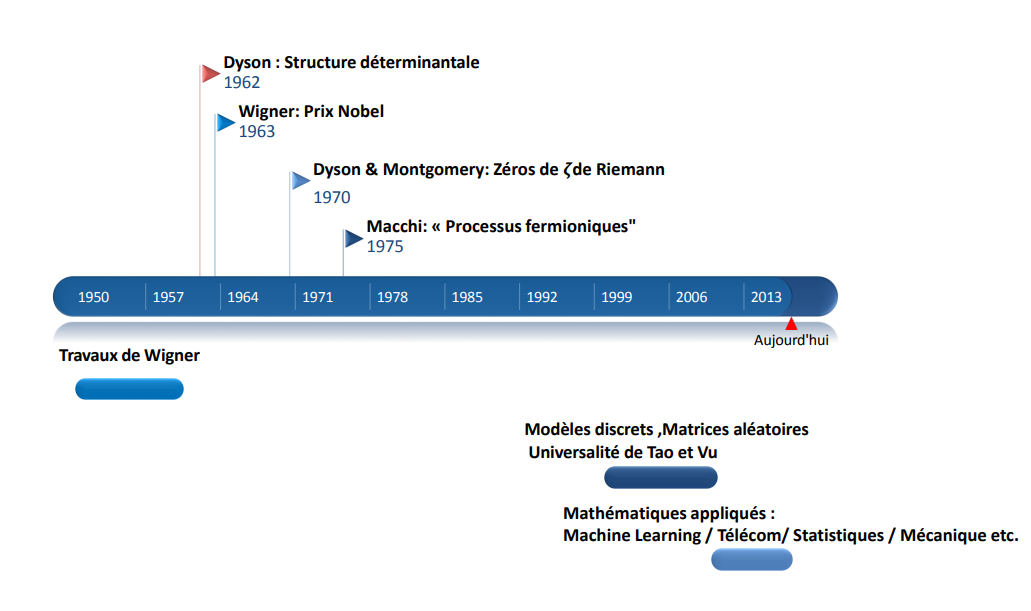
\includegraphics[scale=0.4]{Capture}
\end{frame}
\begin{frame}{Plan}
     \tableofcontents[
    hideothersubsections, 
    sectionstyle=show,
]
\end{frame}



\section{Objects combinatoires}
\begin{frame}{Plan}
\tableofcontents[currentsection,currentsubsection,
    hideothersubsections, 
    sectionstyle=show/shaded,
]
\end{frame}

\subsection{Plus longue sous-suite croissante}
\begin{frame}{Plus longue sous-suite croissante}
\begin{itemize}

\item $\mathfrak{S_n}$ : Le groupe symétrique d'ordre $n$ (l'ensemble des permutations de $\{1,2,\dots,n\}$).
\\ 
\item $i_1<i_2<\dots<i_k$ est une sous-suite croissante de longueur $k$ si $\sigma(i_1)<\sigma(i_2)\dots\sigma(i_k)$.

\item $\ell(\sigma)$  la longueur de la plus longue sous suite croissante
\item Exemple \begin{equation*}\sigma=\begin{pmatrix}
 1& 2 & 3 & 4 & 5 \\ 
 5& 3 & 1 & 2 & 4 
\end{pmatrix}
\end{equation*}
$\ell(\sigma)=3$.

\end{itemize}
\end{frame}
\subsection{Correspondance RSK}

\begin{frame}{Tableaux de Young}
   \begin{definition}[Diagrammes de Young]
   $\lambda=(\lambda_i)_{i\geq1} \in \mathbb{N}^{\mathbb{N}^*}$ est un diagramme de Young de taille $n$ si 
   \begin{itemize}
       \item $\forall i\geq1, \  \lambda_{i+1}\leq \lambda_i$
       \item $\sum_{i=1}^\infty \lambda_i=n$
   \end{itemize}
   \end{definition}
   Exemple : les diagrammes de Young de taille 3 sont $(3,\underline{0}),(2,1,\underline{0}),(1,1,1,\underline{0})$
   \\   ou$\left(\yng(3),\yng(2,1),\yng(1,1,1)\right)$
   
 
\end{frame}
\begin{frame}{Tableau de Young}
    \begin{definition}[Tableau de Young]
    Un tableau de Young de forme $\lambda$ est un remplissage du diagramme de Young $\lambda$ avec les entrées $\{1,2,\dots,n\}$ strictement croissant sur chaque ligne et chaque colonne. 
    \end{definition}
    Exemple : les tableaux de Young de forme $\yng(3,1)$ sont $\young(123,4),\young(124,3),\young(134,2)$. 
\end{frame}


\section{Cas uniforme}
\begin{frame}{Plan}
\tableofcontents[currentsection,currentsubsection,
    hideothersubsections, 
    sectionstyle=show/shaded,
]
\end{frame}
\subsection{correspondance de Robinson-Schinsted}
\begin{frame}{correspondance de Robinson-Schinsted}
    
\end{frame}

\subsection{Conjecture d'Ulam}
\begin{frame}{test}
    
\end{frame}

\subsection{Theorème de Baik Deift Johannson}
\begin{frame}{test}
    
\end{frame}
\section{Universalité}
\begin{frame}{Plan}
\tableofcontents[currentsection,currentsubsection,
    hideothersubsections, 
    sectionstyle=show/shaded,
]
\end{frame}
\end{document}